%!TEX root = ..\Main.tex
\section{Results}\todo{TJEK OM DETTE ER TILFÆLDET FOR ALT DET DER ER SKREVET}
The data is calculated for 35 of the test participants, because 4 was removed due to faulty data on one or more of the sensors.	
A total of x. events were encountered and the average length of a test were x.
%Random ratio - 37,52
Graph x.x.x and. x shows the scatter plot of EHR and FCR for the different sensors. 
Graph x.x.x and. x shows the scatter plot of precision and FCR for the different sensors. Where the average for the different Nu-values is the bordered circles.

%\begin{figure}[h!]
%  \begin{minipage}[t]{0.5\textwidth}
%    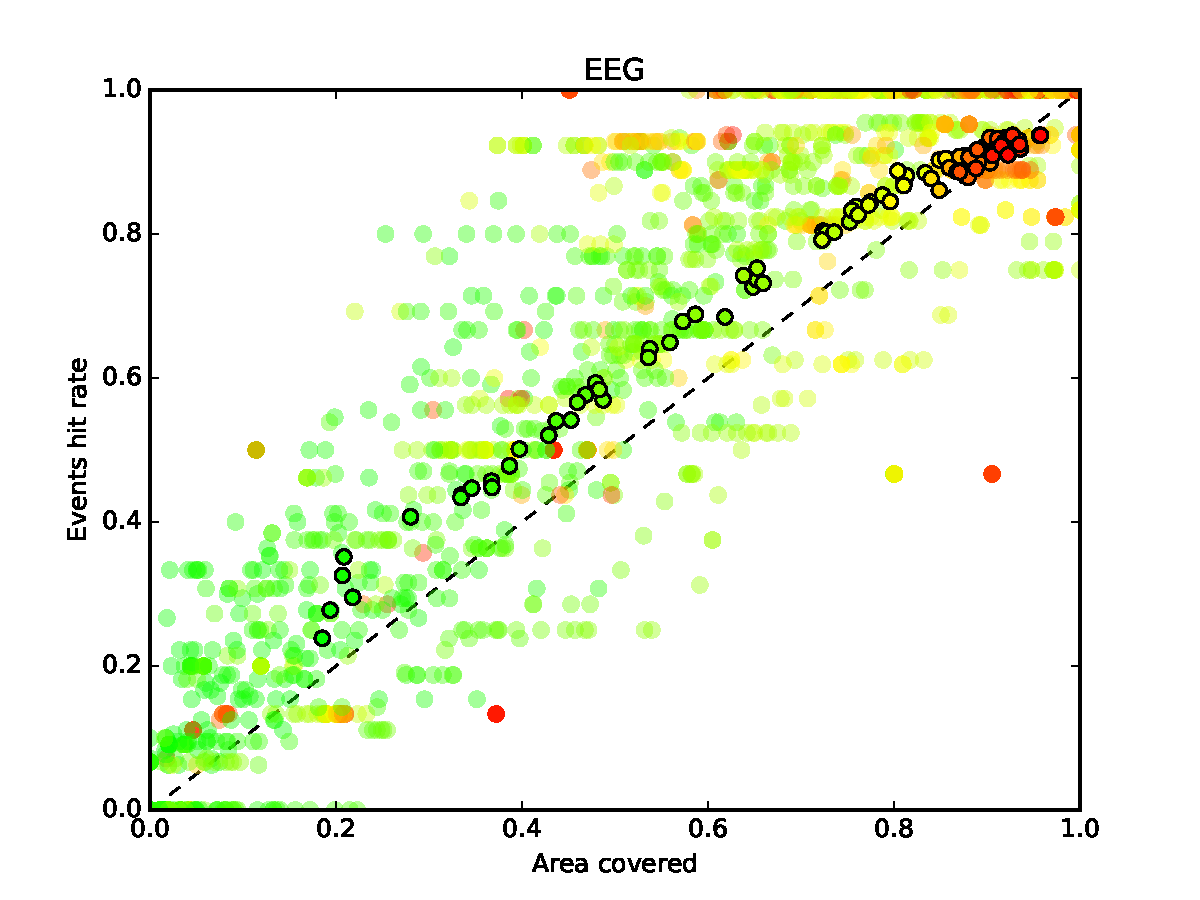
\includegraphics[width=\linewidth,keepaspectratio=true]{graphics/graphs/short/area_covered-events_hit_rate-CovNu-EEG.pdf}
%    \caption{Figura experimental}
%    \label{fase1}
%  \end{minipage}
%  \hspace*{\fill} % it's important not to leave blank lines before and after this command
%  \begin{minipage}[t]{0.5\textwidth}
%    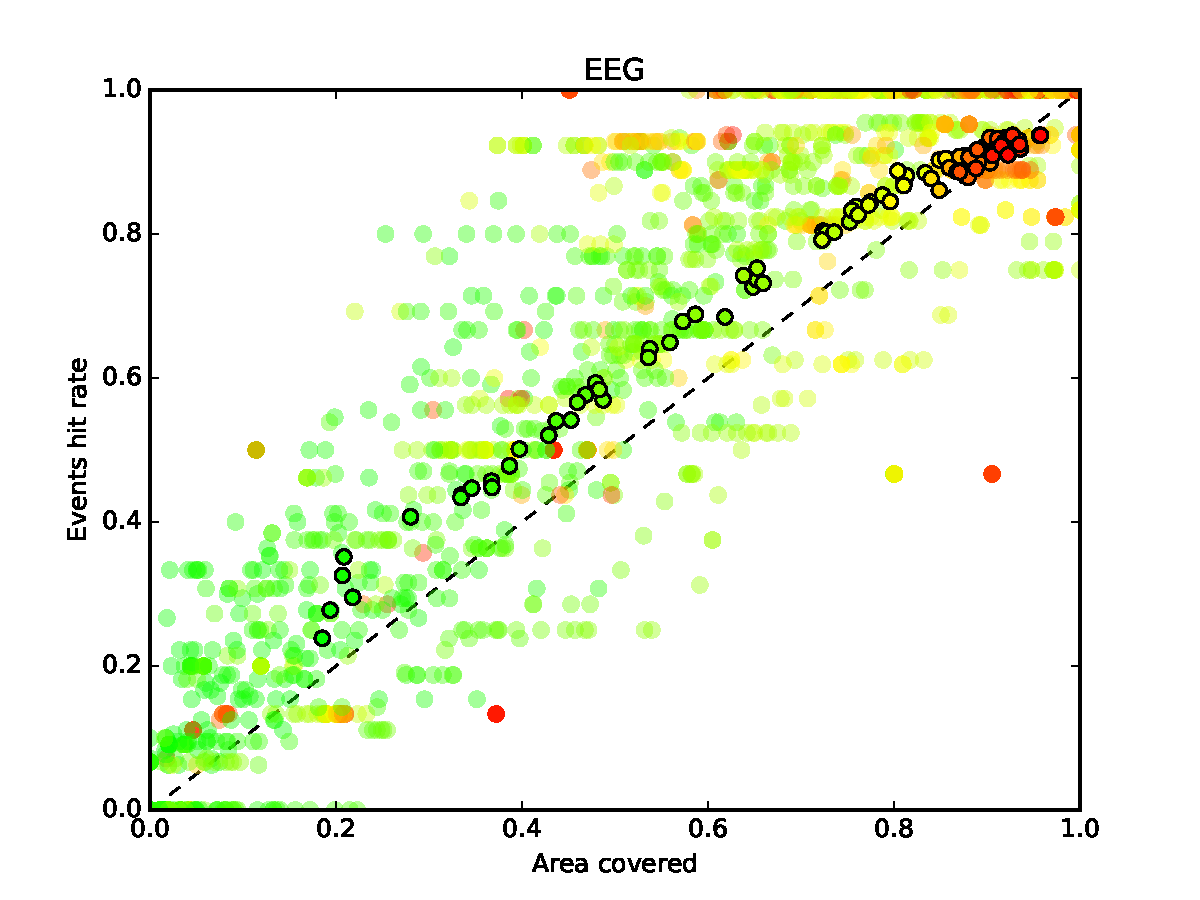
\includegraphics[width=\linewidth,keepaspectratio=true]{graphics/graphs/short/area_covered-events_hit_rate-CovNu-EEG.pdf}
%    \caption{Altra figura experimental}
%    \label{fase2}
%  \end{minipage}
%\end{figure}

\textbf{Sensors likeness and differences}\\
The result from face\todo{Ved ikke om vi bruger face konsistent igennem hele rapporten}, HR, and GSR machines show in general many similar trait.
As seen in Figure x,x,x and x, the Face, HR, and EE machines all shows precision above random guessing at low nu values, and as expected closes in on the random guessing (37,52\%), as higher as the Nu value gets. Meaning if you want a classifier that has a reasonable precision but with false positives, a lower Nu value would be applicable. However the GSR only slightly excite the random ratio at the Nu-value 0.09 and above.
These finding indicates that sensors is not only random guesses but can give a moderately qualified answer to where usability problems can be found.

Looking at graphs x.x.x., and x it can be seen that choosing a higher Nu value for your classifier can yield interesting propositions if the classifier should cover as many problems as possible while minimizing the area wrongly covered.
In other words if one aim is to hit all the events a high Nu value must be chosen, and it comes with the trade-off of place more anomalies outside the events. 
While the GSR and the HR both have a smooth curve through the averages of which indicates a stable classifier, and Face seem to be more unstable in its relation between EHR and FCR. However Face seems to regain some of its stability with higher Nu values. The EEG deviate from the other by already at low values creating many low values, 

All the graph reveals that on across all the test participants no golden Nu-value when trying to detect usability problems is present, but they also show the sensors shows sign of being able to detect when a test participant encounters a usability problems.
The results also showed 
